\section{Izgled završnog rada}

Završni rad se sastoji od praktičnog i pisanog dijela. U praktičnom dijelu studenti formuliraju i rješavaju zadatak. U pisanom dijelu rada 
studenti opisuju odabrane tehnologije, principe i svoja rješenja zadataka.
\subsection{Struktura završnog rada}

Završni rad treba biti strukturiran na sljedeći način:
\begin{itemize}
 \item naslovnica,
 \item sadržaj,
 \item uvod,
 \item opis korištenih tehnologija,
 \item opis izrade praktičnog dijela,
 \item zaključak,
 \item popis literature.
\end{itemize}

Završni rad počinje naslovnicom. Na naslovnici se nalaze sljedeći podaci:
\begin{itemize}
 \item naziv ustanove,
 \item naslov završnog rada,
 \item ime studenta,
 \item ime mentora, te
 \item datum izrade (mjesec i godina).
\end{itemize}

\subsection{Naslovnica i sadržaj}
Detaljni izgled naslovnice nalazi se na stranicama ~\href{http://oss.unist.hr/index.php/odjel/propisi-i-dokumenti/243-pravilnik-o-izradi-i-obrani-zavrsnog-rada}{\texttt{oss.unist.hr}}.
Naslovnica nije numerirana.  
Sadržaj je numeriran rimskim brojevima. Sve ostale stranice u završnom radu trebaju biti numerirane arapskim brojevima. 
Sadržaj treba biti automatski generiran.

\begin{comment}
 
Ukoliko se dokument dvostrano printa vrijedi:
\begin{itemize}
\item Nakon naslovne stranice slijedi prazna stranica (zbog dvostranog ispisa). 
\item Ukoliko sadržaj zauzima neparan broj stranica, nakon sadržaja ostaviti jednu praznu stranicu.
\end{itemize}



Završni rad se ne printa dvostrano.


Počevši od uvoda svaka stranica mora imati zaglavlje u kojem je označen broj stranice i poglavlje (primjer u ovom dokumentu). 

Na neparnim stranicama broj stranice treba biti na desnoj strani, a na parnim stranicama na lijevoj strani.
\end{comment}
Na kraju završnog rada treba biti popis literature ili web izvora.
\subsection{Format teksta}

\begin{itemize}
 \item Format papira A4.
 \item Font times ili neki slični, veličina 11pt ili 12pt.
 \item Margine oko 2.5 cm sa svake strane. 
 \item Obostrano poravnanje.
 \item Prored teksta 1.2 (\textit{line spacing}).
 \item Između paragrafa treba biti veći razmak.
 \item Na početku paragrafa redak je malo uvučen (nije obavezno).
 \end{itemize}

\subsection{Slike, tablice i k\^od}
Slike i tablice trebaju biti označene brojevima npr. "Slika 1: Primjer Xfce radne okoline". Svaka slika treba biti referirana na barem jednom mjestu u tekstu. 
Primjerice, na slici~\ref{fig:xfce} je prikazan jedan od bezbroj mogućih izgleda radne okoline.
\\[\intextsep]
\begin{minipage}{\linewidth}
\centering%
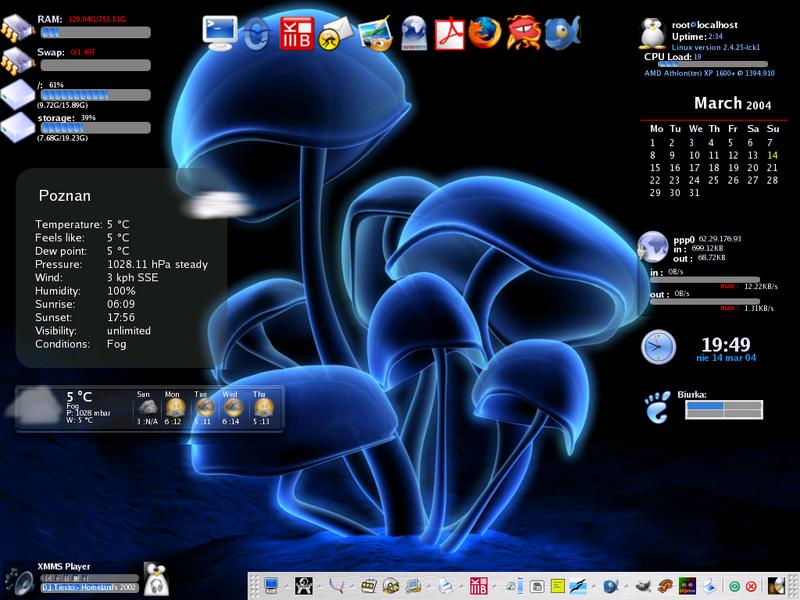
\includegraphics[width=0.8\linewidth,clip=]{xfce.jpg}%
\figcaption{Primjer Xfce radne okoline}%
\label{fig:xfce}%
\end{minipage}
\\[\intextsep]

%\begin{figure}[ht]
%  \centering
%  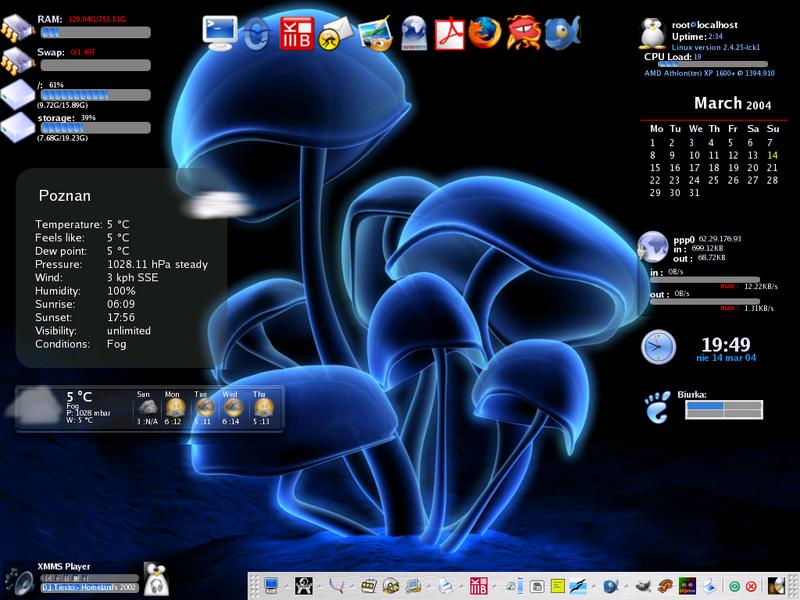
\includegraphics[width=0.5\textwidth]{xfce.jpg}  
%  \caption{Xfce radna okolina}
%  \label{fig:xfce}  
%\vspace{-10pt}
%\end{figure}

K\^od se piše fontom u kojem su sva slova jednake širine. Primjer takvog fonta je \texttt{courier}. Listu slobodnih \textit{monospace} fontova možete naći na stranicama \url{http://www.fontsquirrel.com/fonts/list/classification/monospaced}. 
Veličina slova treba biti nešto manja nego u običnom tekstu. Primjer k\^oda je dan u ispisu~\ref{program}.
%
%\begin{lstlisting}
%#! /bin/bash
%# skripta za prebacivanje "layout-a" tipkovnice
%setxkbmap $1
%echo Prebacili ste na $1 tipkovnicu.
%\end{lstlisting}
%\caption{Skripta za mijenjanje položaja tipkovnice}
%\label{fig:program}
%\end{figure}

\begin{lstlisting}[caption={Skripta za mijenjanje rasporeda tipki tipkovnice}, label=program]
#! /bin/bash
# skripta za mijenjanje "layout-a" tipkovnice
setxkbmap $1
echo Prebacili ste na $1 tipkovnicu.
\end{lstlisting}



\subsection{Formatiranje dokumenta}

Bez obzira koji se alati za formatiranje teksta koriste, završni rad mora biti korektno formatiran. U slučaju da se koristi Microsoft Word, 
dobra preporuka je da se unaprijed definira 
stil dokumenta. Dakle, unaprijed se definiraju veličine naslova, podnaslova, fontovi i slično. Bitno je da određeni stil prati cijeli završni rad. 
Primjerice, ako se koristi 
uvučeni redak na početku prvog paragrafa, onda redak mora biti uvučen na početku svakog paragrafa.
U slučaju da student želi koristiti \LaTeX, može dobiti predložak ovog dokumenta za pomoć pri izradi rada.
\subsection{Pravopis i gramatika}

Studenti su obavezni predati pravopisno i gramatički korektan rad. Završni radovi koji nisu ispravno napisani neće biti mentorirani. Provjera ispravnosti riječi može se obaviti putem stranice \href{http://hjp.novi-liber.hr/}{hrvatskog jezičnog portala}. Pravila hrvatskog pravopisa mogu se naći na stranicama \href{www.pravopis.hr}{www.pravopis.hr}. Među pravilima treba obratiti pozornost na pisanje tuđica koje su uobičajene u pisanju radova iz područja računarstva. Osim toga, obavezna je i provjera teksta \textit{spell checkerom} hrvatskog jezika. Ukoliko nemate \textit{spell checker}, na stranicama \url{https://hacheck.tel.fer.hr/} nalazi se online \textit{spell checker}.
\subsection{Kratice}

Prilikom prvog pojavljivanja, kratice u tekstu se opisuju, a u daljnjem tekstu se koriste bez ponovnog opisa. Popis kratica treba biti dodan na kraj završnog rada.
\subsection{Strane riječi}
U završnom radu koristi se hrvatski jezik kada za određenu riječ postoji hrvatski prijevod. Ukoliko korištenje takve hrvatske riječi nije 
uobičajeno u praksi ili autori rada ne 
poznaju odgovarajuću hrvatsku riječ, ostavlja se strana riječ napisana \textit{u kurzivu}.

Kada se prvi put uvodi pojam na hrvatskom jeziku, potrebno je u zagradama navesti i originalnu riječ. Npr. jezgra (engl.~\textit{kernel}) operacijskog sustava.  
\subsection{Stil}

Završni rad se piše u neutralnom stilu i bezlično npr. "ispitivanje je pokazalo...". 
Treba izbjegavati prvo lice jednine i prvo lice množine. 
\subsection{Citati i popis literature}

Svi citati (doslovno prepisani dijelovi drugog autora ili izjave) označavaju se navodnicima i
određuju brojčano uz objašnjenje u fusnoti (bilješkama ispod teksta o autoru navoda i djelu, godini izdanja, izdavaču i broju stranice).

U popisu literature treba navesti literaturu koja se koristila za izradu rada, te popis web stranica. Popisi trebaju biti 
grupirani i to tako da se prvo navede popis literature, a onda 
popis web stranica sa datumom zadnjeg pristupanja stranici.
Sama literatura navodi se kako slijedi:
\begin{enumerate}
\item 
Prezime autora, inicijal imena: Naslov knjige, izdavač, mjesto i godina izdavanja
\item Prezime autora, inicijal imena: Naslov rada, naziv skupa, časopisa ili zbornika radova,
mjesto i godina objavljivanja
\item Prezime autora, inicijal imena: Naslov rada, web stranica objavljivanja
\end{enumerate}

\subsection{Plagiranje}

Citiranje je doslovno preuzimanje dijelova drugog rada. Citira se u navodnicima uz fusnotu u kojoj se nalazi podatak o tome koji se rad citira. 
Svako drugačije preuzimanje dijelova teksta 
smatra se plagijatom i nije dopušteno u izradi završnog rada. 

S druge strane parafraziranje je vlastitim riječima opisan dio drugog rada. 
I u tom slučaju potrebno je navesti izvor 
parafraziranog teksta. Doslovno prevođenje sa stranog jezika smatra se plagijatom. Ukoliko student pošalje rad za koji mentor utvrdi da je plagiran u bilo kojem dijelu teksta, mentor neće mentorirati ni ispravljati ostatak završnog rada. 

\subsection{Imenovanje dokumenta}

Završni rad predaje se u pdf formatu. Ukoliko se tijekom izrade šalje na provjeru mentoru, svaka nova verzija dokumenta treba biti 
ispravno numerirana kako bi se iz imena 
dokumenta lako moglo odrediti da li je dokument noviji od prethodno poslanih. Npr. pet dokumenata koji se šalju na čitanje mogu biti 
imenovani na sljedeći način:
\\
\texttt{prezime\_zavrsni\_1.0.pdf}\\
\texttt{prezime\_zavrsni\_1.1.pdf}\\
\texttt{prezime\_zavrsni\_1.2.pdf}\\
\texttt{prezime\_zavrsni\_1.3.pdf}\\
\texttt{prezime\_zavrsni\_2.0.pdf}\\
Nula na kraju imena (1.0, 2.0 itd) označava verzije sa bitnim izmjenama, dok se verzije sa manjim izmjenama označavaju ostalim brojevima (1.1, 1.2, 2.1 itd). 

Osim navedene mogućnosti numeriranja, postoji mogućnost da se završni rad stavi na neki od repozitorija za kolaboraciju (\textit{github, subversion, cvs}). Odabir takve mogućnosti je poželjan.

\subsection{Dodatne napomene}

Iza znaka interpunkcije (točka, zarez, upitnik, uskličnik i slično) stavlja se razmak. Razmak dolazi i prije otvorene zagrade, ali ne i nakon otvorene zagrade i prije zatvaranja zagrade. 
Nakon zagrade ponovo se stavlja razmak.
